\chapter{Architecture}

\section{Rules, rule-sets, and rule-bases}

Within Drools, the concepts of rules, rule-sets and rule-bases
are directly modelled by the classes \indexClass{Rule},
\indexClass{RuleSet} and \indexClass{RuleBase}.  A \indexClass{Rule}
may be a member of multiple \indexClass{RuleSet}s, and multiple
\indexClass{RuleSet}s may be active within a given
\indexClass{RuleBase}.

\subsection{\indexClass{Rule}, \indexClass{Condition} and \indexClass{Consequence}}

A single \indexClass{Rule} may have one-or-more
\indexClass{Condition}s associated with it.  Each condition 
must be met before the rule is considered to be activated.
Once activated the rule's \indexClass{Consequence} is a
candidate for being fired.  In pattern parlance, the
\indexClass{Condition} class is simply a \emph{predicate
object}\index{predicate object} which evaluates itself against
the known facts to return a boolean value of either \emph{true}
or \emph{false}.  The \indexClass{Consequence} class is likewise
simply a \emph{functor} which objectifies a function and performs
an arbitrary task when executed.

\begin{figure}[h]
  \begin{center}
  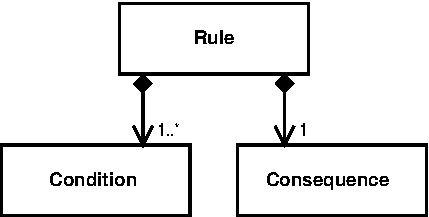
\includegraphics{rule}
  \end{center}
  \caption{Object model for \class{Rule}, \class{Condition} and \class{Consequence}}
\end{figure}

\subsection{\indexClass{RuleSet}}

A \indexClass{RuleSet} is simply a collection of \indexClass{Rule}s.
It serves only to associate a group of rules with one another so that
they may be worked with as a set.

\begin{figure}
  \begin{center}
  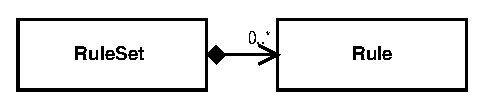
\includegraphics{ruleset}
  \end{center}
  \caption{Object model for \class{RuleSet} and \class{Rule}}
\end{figure}

\subsection{\indexClass{RuleBase}}

A \indexClass{RuleBase} is an \emph{active} collection of
\indexClass{RuleSet}s.  A \indexClass{RuleBase} contains rules
that are all considered to be in effect for a given set of
knowledge.  Multiple \class{RuleSet}s may be a part of a 
given \class{RuleBase}.

\begin{figure}
  \begin{center}
  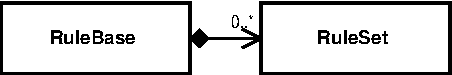
\includegraphics{rulebase}
  \end{center}
  \caption{Object model for \class{RuleBase} and \class{RuleSet}}
\end{figure}

\section{Knowledge}

The set of knowledge that is examined is modelled by the class
\indexClass{WorkingMemory}, which is backed by a particular
\indexClass{RuleBase}.  It is through the \indexClass{WorkingMemory}
that knowledge is \emph{asserted}, \emph{retracted} and
\emph{modified}.
Each \class{WorkingMemory} is backed by exactly one
\indexClass{RuleBase} which determines which rules are evaluated
as knowledge is manipulated.

\begin{figure}
  \begin{center}
  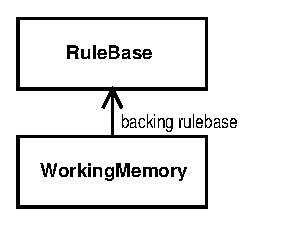
\includegraphics{workingmemory}
  \end{center}
  \caption{Object model for \class{WorkingMemory} and \class{RuleBase}}
\end{figure}

\clearpage

\section{Complete Model}

\begin{figure}[h]
  \begin{center}
  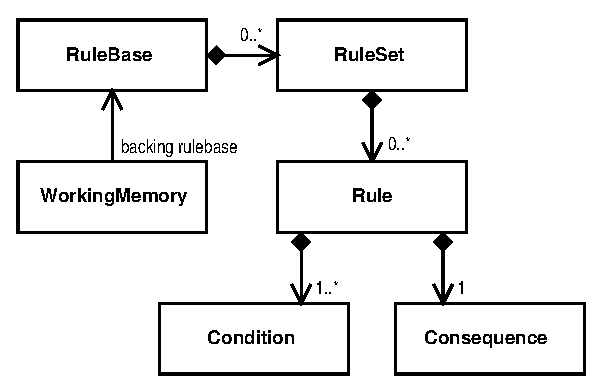
\includegraphics{architecture}
  \end{center}
  \caption{Complete object model}
\end{figure}
